

\section{Experiments}
\label{sec:experiments}
We implement \method~using the verl codebase \citep{sheng2024hybridflow}, using vLLM \citep{kwon2023efficient} for inference and FSDP \citep{zhao2023pytorch} for training. We use Qwen3-8B-Instruct (Qwen/Qwen3-8B) \citep{yang2025qwen3technicalreport} as the base model. We sample 5 responses using the initial policy for each prompt, precompute the reference responses using the reward model \texttt{Skywork-Reward-V2-Llama-3.1-8B-40M} \citep{liu2025skywork}, and store them as part of the dataset. During training, we sample 6 role-response pairs from the model for each prompt as a response group, and embed them using \texttt{all-MiniLM-L6-v2} \citep{wang2020minilmdeepselfattentiondistillation}. Our training has two generation settings: thinking-enabled and thinking-disabled. Quality and diversity metrics are computed only over the final answer, with the thinking trace masked out, throughout the training-time reward computation and evaluation. We include more implementation details in Appendix \ref{appx:implementation}.

\paragraph{Baselines.}
\label{subsec:baselines}
Given that \method{} is a training-based method, the most direct comparisons are training-time approaches. Both \textbf{DARLING}~\citep{li2025jointlyreinforcingdiversityquality} and \textbf{DivPO} \citep{lanchantin2025diverse} update model parameters to jointly optimize for diversity and quality during the training time. \textbf{DivPO} is a preference-optimization (DPO) method that constructs response preference pairs by selecting rare, high-quality responses as preferred and common, low-quality ones as rejected. \textbf{DARLING} optimizes an online RL objective with a learned diversity signal. We trained two versions of DARLING: one using our mixture data (Training Data, below) and one using their specified recipe (10k prompts subsampled from WildChat). On the inference-time side,  we \textbf{repeatedly sample} the base model $k$ times per prompt without role conditioning, testing whether stochastic decoding alone suffices. We also compared with \textbf{\ssot}~\citep{Misaki2026}, a representative prompting method that induces diversity by injecting random string seeds in the thinking tokens as an entropy source. Notably, inference-time and training-time methods are complementary. We can apply inference-time methods to \method{} at decoding time to further amplify diversity improvements.


%\textbf{Naive Role Prompting} applies the same role codes to the frozen model without role-diversity training, isolating the contribution of training from role labels alone. \textbf{Quality-Only RL} trains with the quality reward and penalties with $\lambda_d = 0$, ablating the diversity term.
%\textbf{Diversity-Only RL} trains with the diversity reward and penalties with $\lambda_q = 0$, ablating the quality term.
%\textbf{No-Role Diversity RL} trains with the full QGDR objective but without role conditioning, testing whether an unconditioned policy can learn diverse behavior without explicit control codes.
%We include DARLING because it is the closest training-time baseline for jointly reinforcing quality and diversity. 
%When possible, we use the official implementation; otherwise, we reproduce the reward structure in the same training stack used for our method.

\paragraph{Training Data.}
\label{subsec:training data}
The training set contains 10K prompts, constructed from a 4:1 mixture of uniformly sampled Tulu3-SFT-Mix prompts~\citep{lambert2024tulu3} and Infinite-Chat dataset~\citep{jiang2025artificialhivemindopenendedhomogeneity}. This mixture balances quality and diversity: Tulu3-SFT-Mixture provides instruction-following prompts that preserve response quality, while Infinite-Chat encourages open-ended exploration.


\paragraph{Generative Diversity Evaluation.}
To evaluate generative diversity, we focus on two application domains where multiple distinct high-quality outputs are desirable: \textbf{scientific ideation} and \textbf{creative writing}. We evaluate all methods under the \textbf{diverse mode}, with the role code injected into the system prompt. Notably, none of the evaluation datasets below overlap with our training data, so strong performance here reflects genuine transfer rather than in-domain memorization. In the \textbf{science ideation} domain, we adapt HypoBench~\citep{liu2026hypobenchsystematicprincipledbenchmarking} and PreScience~\citep{Ajith2026} for our cases. In the \textbf{creative writing} domain, we evaluate on NoveltyBench~\citep{zhang2025noveltybenchevaluatinglanguagemodels} and a held-out set of Infinite-Chat~\citep{jiang2025artificialhivemindopenendedhomogeneity}. We describe the adaptation of HypoBench and PreScience to our setting in Appendix~\ref{app:domain application}. We measure output diversity using a comprehensive set of diversity metrics: \textit{semantic-level} (SBERT), \textit{entropy-level} (E-Vendi) \citep{friedman2023vendiscorediversityevaluation}, and \textit{entailment-level} (Discriminator/Disc.), a pairwise classifier trained to predict whether two responses to the same prompt are conceptually distinct (training details in Appendix~\ref{appx:discriminator}).


% \liwei{the hierarchical structure feels wrong of this section. why do we have separate paragraphs for \textbf{HypoBench.} and \textbf{PreScience.} but not the creative writing benchmarks? restructure to make the hierarchy clear }

%For each prompt, we sample multiple responses from the model and report both quality and diversity metrics, allowing us to quantify whether diversity-oriented training improves output variety without degrading general model capability.

%\textbf{NoveltyBench.}
%For each prompt, each system generates $k$ candidates. We follow the benchmark's set-level framing and report Distinct@$k$ and Utility@$k$. Distinct@$k$ measures the number of meaningfully distinct generations in the candidate set, while Utility@$k$ credits responses that are both novel and high quality. We report results on the curated split and, compute permitting, the WildChat split. We use the same $k$ across all systems. If the trained model has fewer roles than $k$, we allocate additional samples evenly across roles.


%\textbf{HypoBench.}
%HypoBench evaluates hypothesis generation, making it a direct test of whether role-conditioned diversity improves scientific exploration. For each task, the model generates a set of candidate hypotheses. We evaluate practical utility, plausibility, generalizability, and hypothesis discovery rate using benchmark-provided metrics and judge-based rubrics. We additionally measure hypothesis-set diversity using embedding distance, semantic clustering, Self-BLEU, and the number of unique valid hypotheses recovered across roles.

\liweiaddressed{The hierarchy of the following paragraphs is a bit confusing. There are two types of benchmarks: general capability, diversity. So the first two paragraphs should lie at the same layer of hierarchy. HypoBench and PreScience are two specific benchmarks for the second type of benchmark. Also, there are two more benchmarks (novelty bench, Infinite-Chat) that are not introduced. Could we have the experiment section to be organized as following: (1) baselines; (2) training data; (3) diversity evaluations (introducing those four benchmarks); (4) general capability benchmarks. Also, we should be informative with the naming of the diversity benchmark. "domain application" feel a bit too genetic.}


\paragraph{General Capability Retention Evaluation.}

\liweiaddressed{add a short sentence to highlight why we need general capability tests.}
To assess whether our method preserves the model's reasoning capability, we evaluate each trained model in the standard single-response setting on a suite of seven widely used benchmarks under the \textbf{standard mode}. Specifically, we use GSM8K~\citep{cobbe2021gsm8k} to evaluate mathematical reasoning; MMLU~\citep{hendryckstest2021}, GPQA~\citep{rein2024gpqa}, and BoolQ~\citep{clark2019boolq} to evaluate broad knowledge and question answering; HellaSwag~\citep{zellers2019hellaswag} to evaluate commonsense inference; TruthfulQA-MC1~\citep{lin2022truthfulqameasuringmodelsmimic} to evaluate truthfulness; IFEval~\citep{zhou2023instructionfollowingevaluationlargelanguage} to evaluate instruction following. We used a max token length of 8192 for the thinking-enabled setting, 2048 for the thinking-disabled setting. 
% \liwei{where do we include these general capability results?}

\liweiaddressed{Can we specify in what mode of the dual mode did we test the general benchmarks on?}




%\textbf{Capability retention.}
%Although diversity is the main target, the model should still behave normally when no role code is supplied. We therefore evaluate no-role performance on closed-form or standard capability benchmarks such as GPQA, GSM8K, MATH-style reasoning, and MMLU-style QA. These results are treated as retention checks rather than the main diversity claim.

%\textbf{Human evaluation.}
%For a subset of NoveltyBench and Infinite-Chat prompts, human annotators compare anonymized response sets. Annotators judge whether the set is more diverse, whether the responses remain useful, and whether any responses are off-task or repetitive. Human judgments are reported separately for diversity and usefulness to avoid rewarding low-quality variation.

%\textbf{Statistical reporting.}
%All main comparisons use prompt-level paired statistics. We report mean scores with bootstrap confidence intervals over prompts. For pairwise system comparisons, we report paired bootstrap differences. For human evaluation, we report preference rates, disagreement rates, and confidence intervals.
\section{Results}
% \begin{figure}[t!]
%     \centering
%     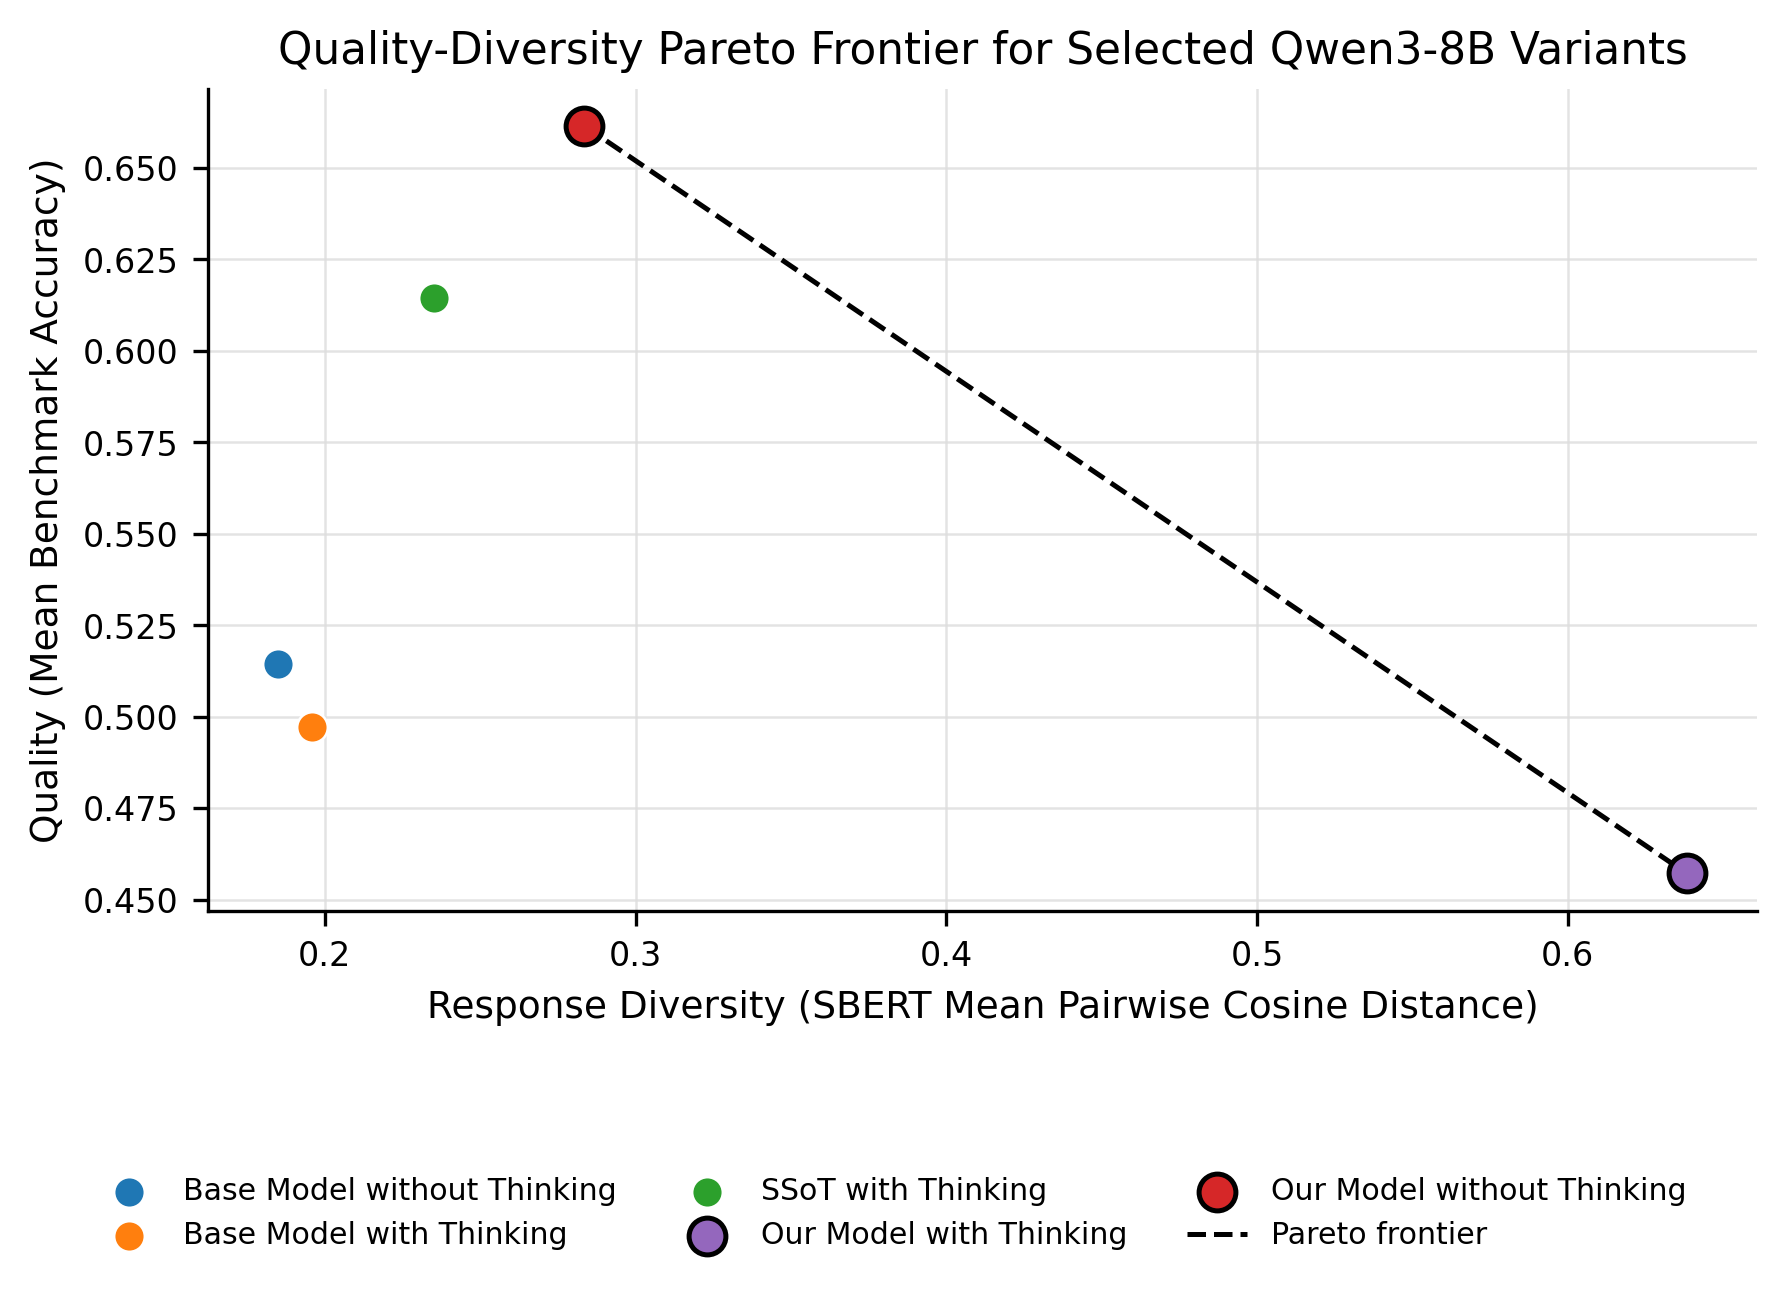
\includegraphics[width=\textwidth]{figures/pareto}
% \vspace{-0.5cm}
% \label{fig:intro}
% \end{figure}

\textbf{Generative Diversity Evaluation.} As shown in Figure~\ref{fig: domain application pareto}a, \method{} Pareto-dominates all baselines on the held-out Infinite-Chat set across every setting (thinking enabled/disabled, different base models), achieving both higher diversity and higher quality simultaneously; the remaining settings are shown in Appendix~\ref{appx:generative diversity evaluation}. We provide a breakdown by individual benchmarks in Table~\ref{tab:domain-app-diversity-main}. Across four domains and three model families, \method{} achieves the best average diversity across all evaluated baselines, while matching or improving quality on most domains except PreScience. Notably, \method{} outperforms all baselines on HypoBench, a scientific ideation task that is out of domain relative to our training set, which primarily consists of standard SFT data and open-ended questions. These results suggest that \method{} enhances general exploration capability across thinking settings and base models, even on out-of-domain topics.

\begin{figure}[ht]
\centering
\begin{minipage}{0.45\linewidth}
  \centering
  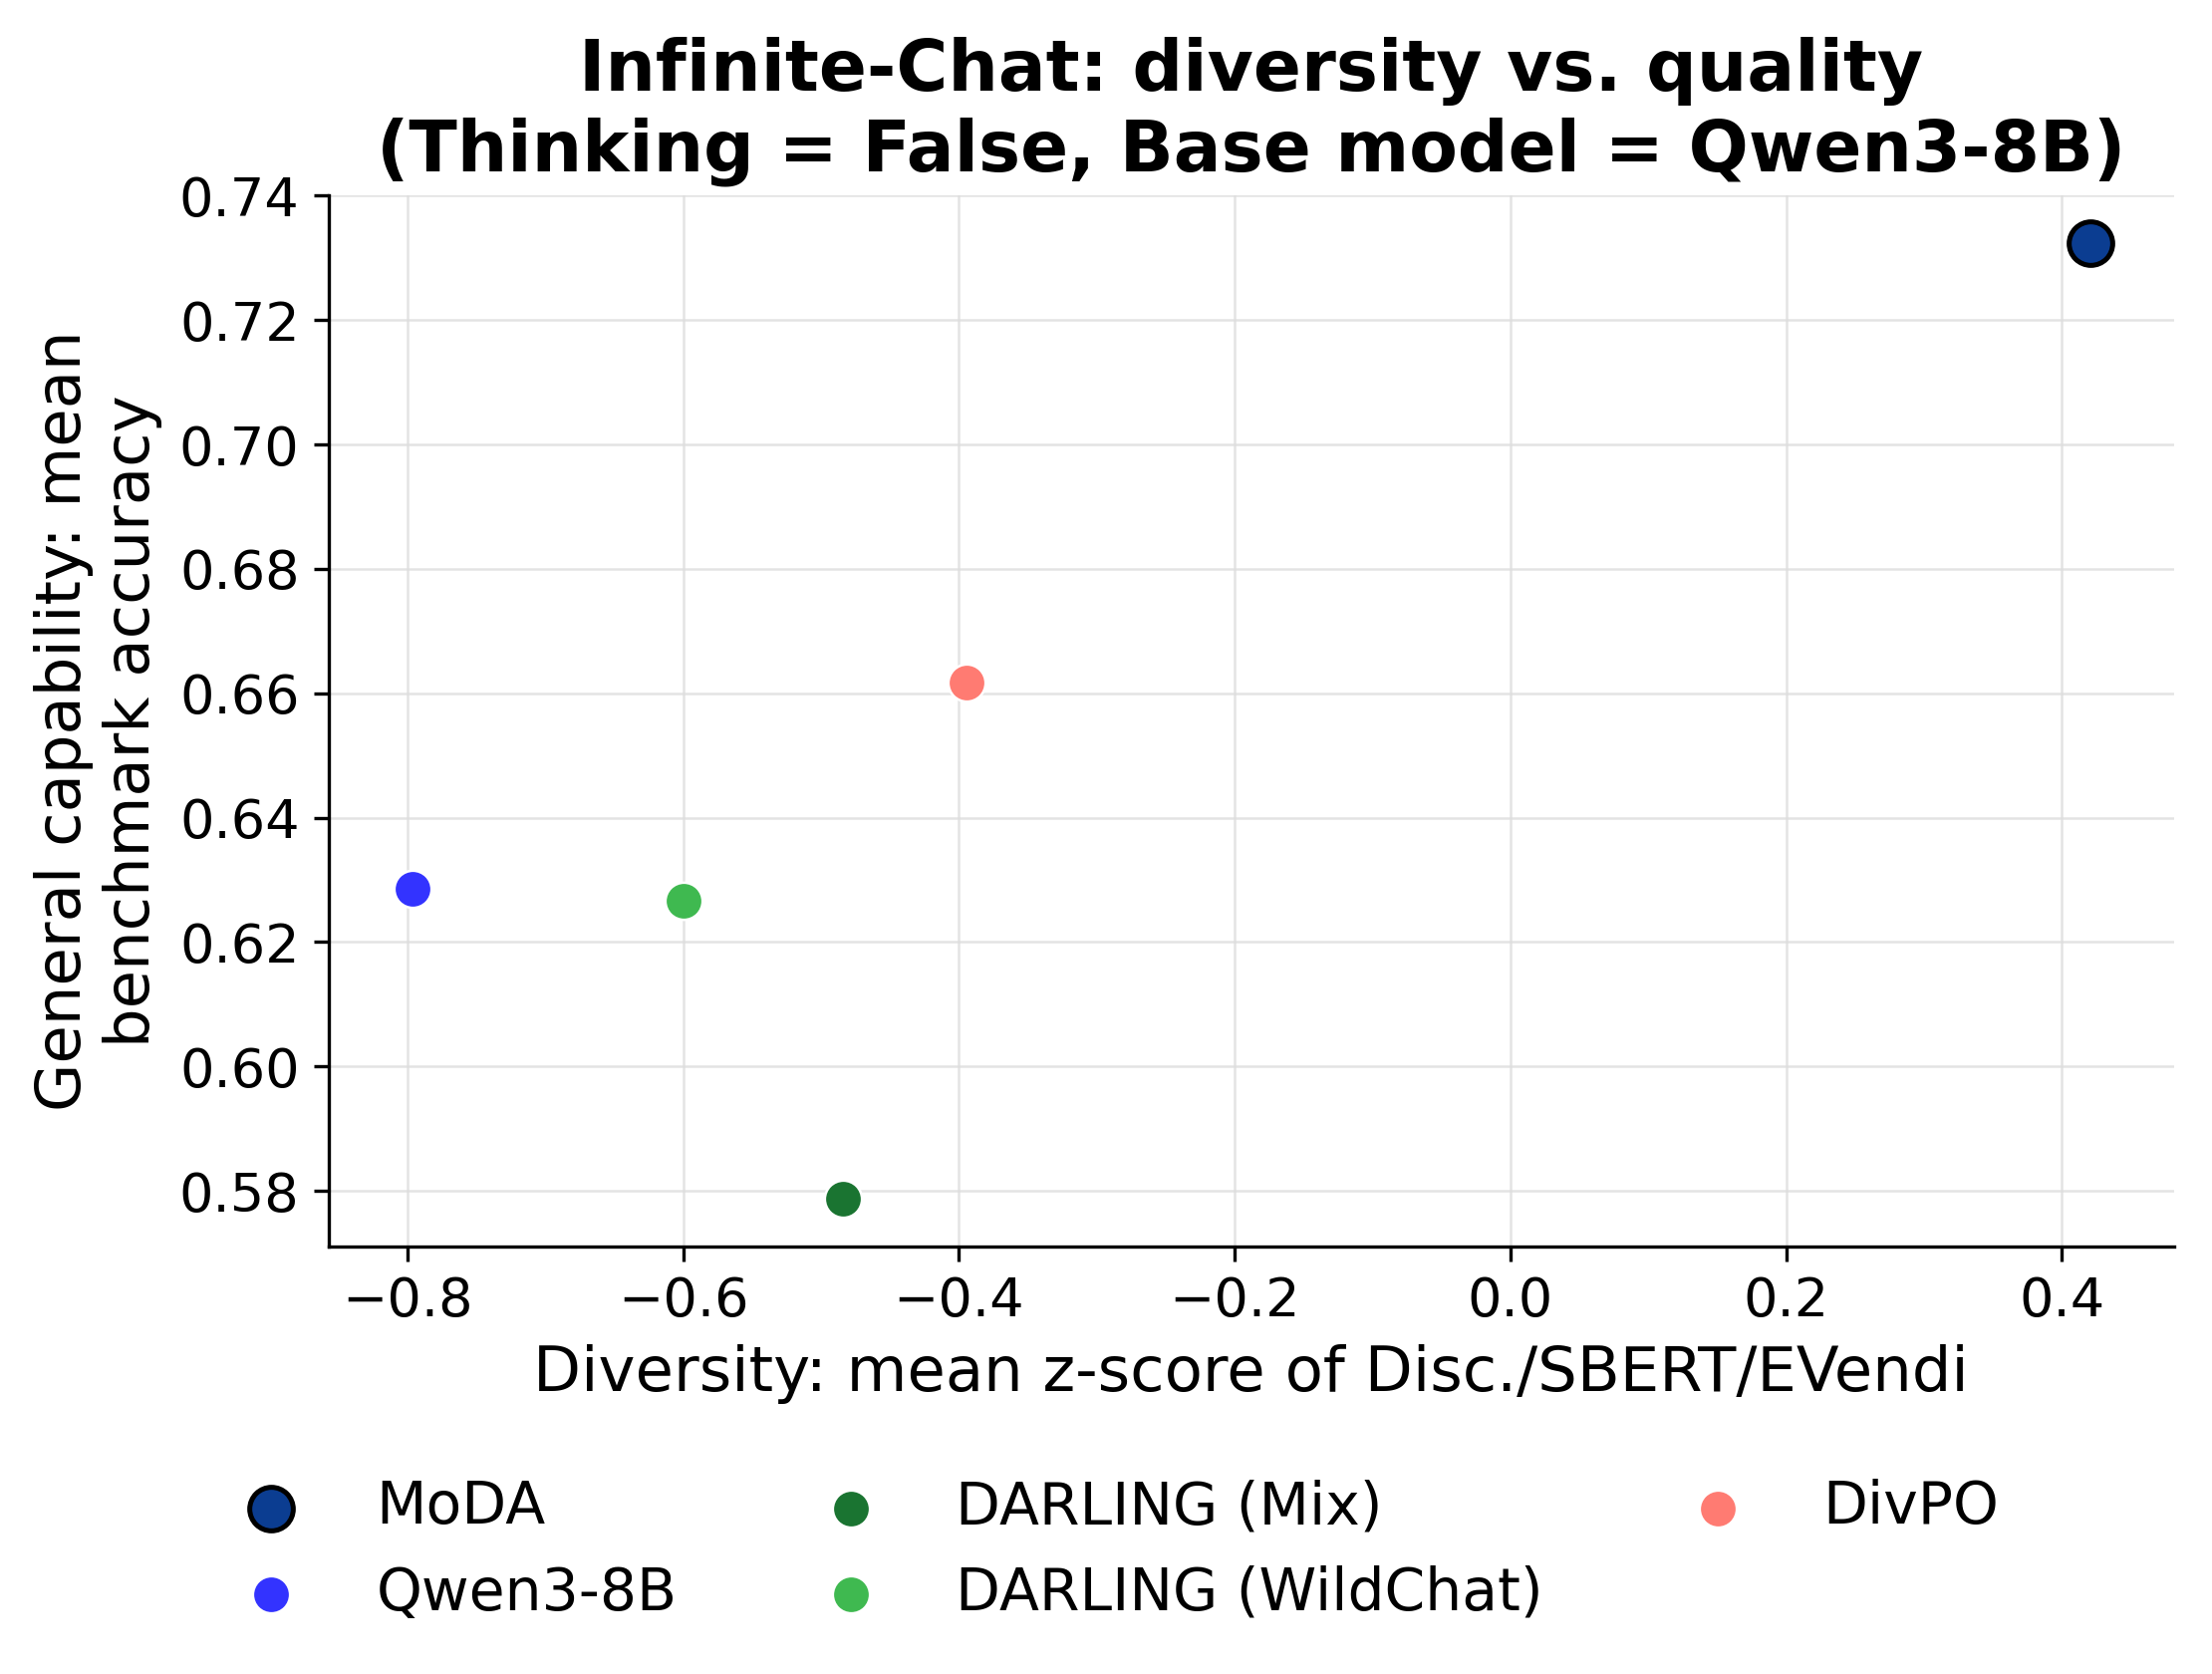
\includegraphics[width=\linewidth]{figures/pareto_infinite-chat_quality_thinking_false_base_model_qwen3-8b_composite.png}
  \small (a) Baselines
  \label{fig: domain application pareto baselines}
\end{minipage}\hfill
\begin{minipage}{0.5\linewidth}
  \centering
  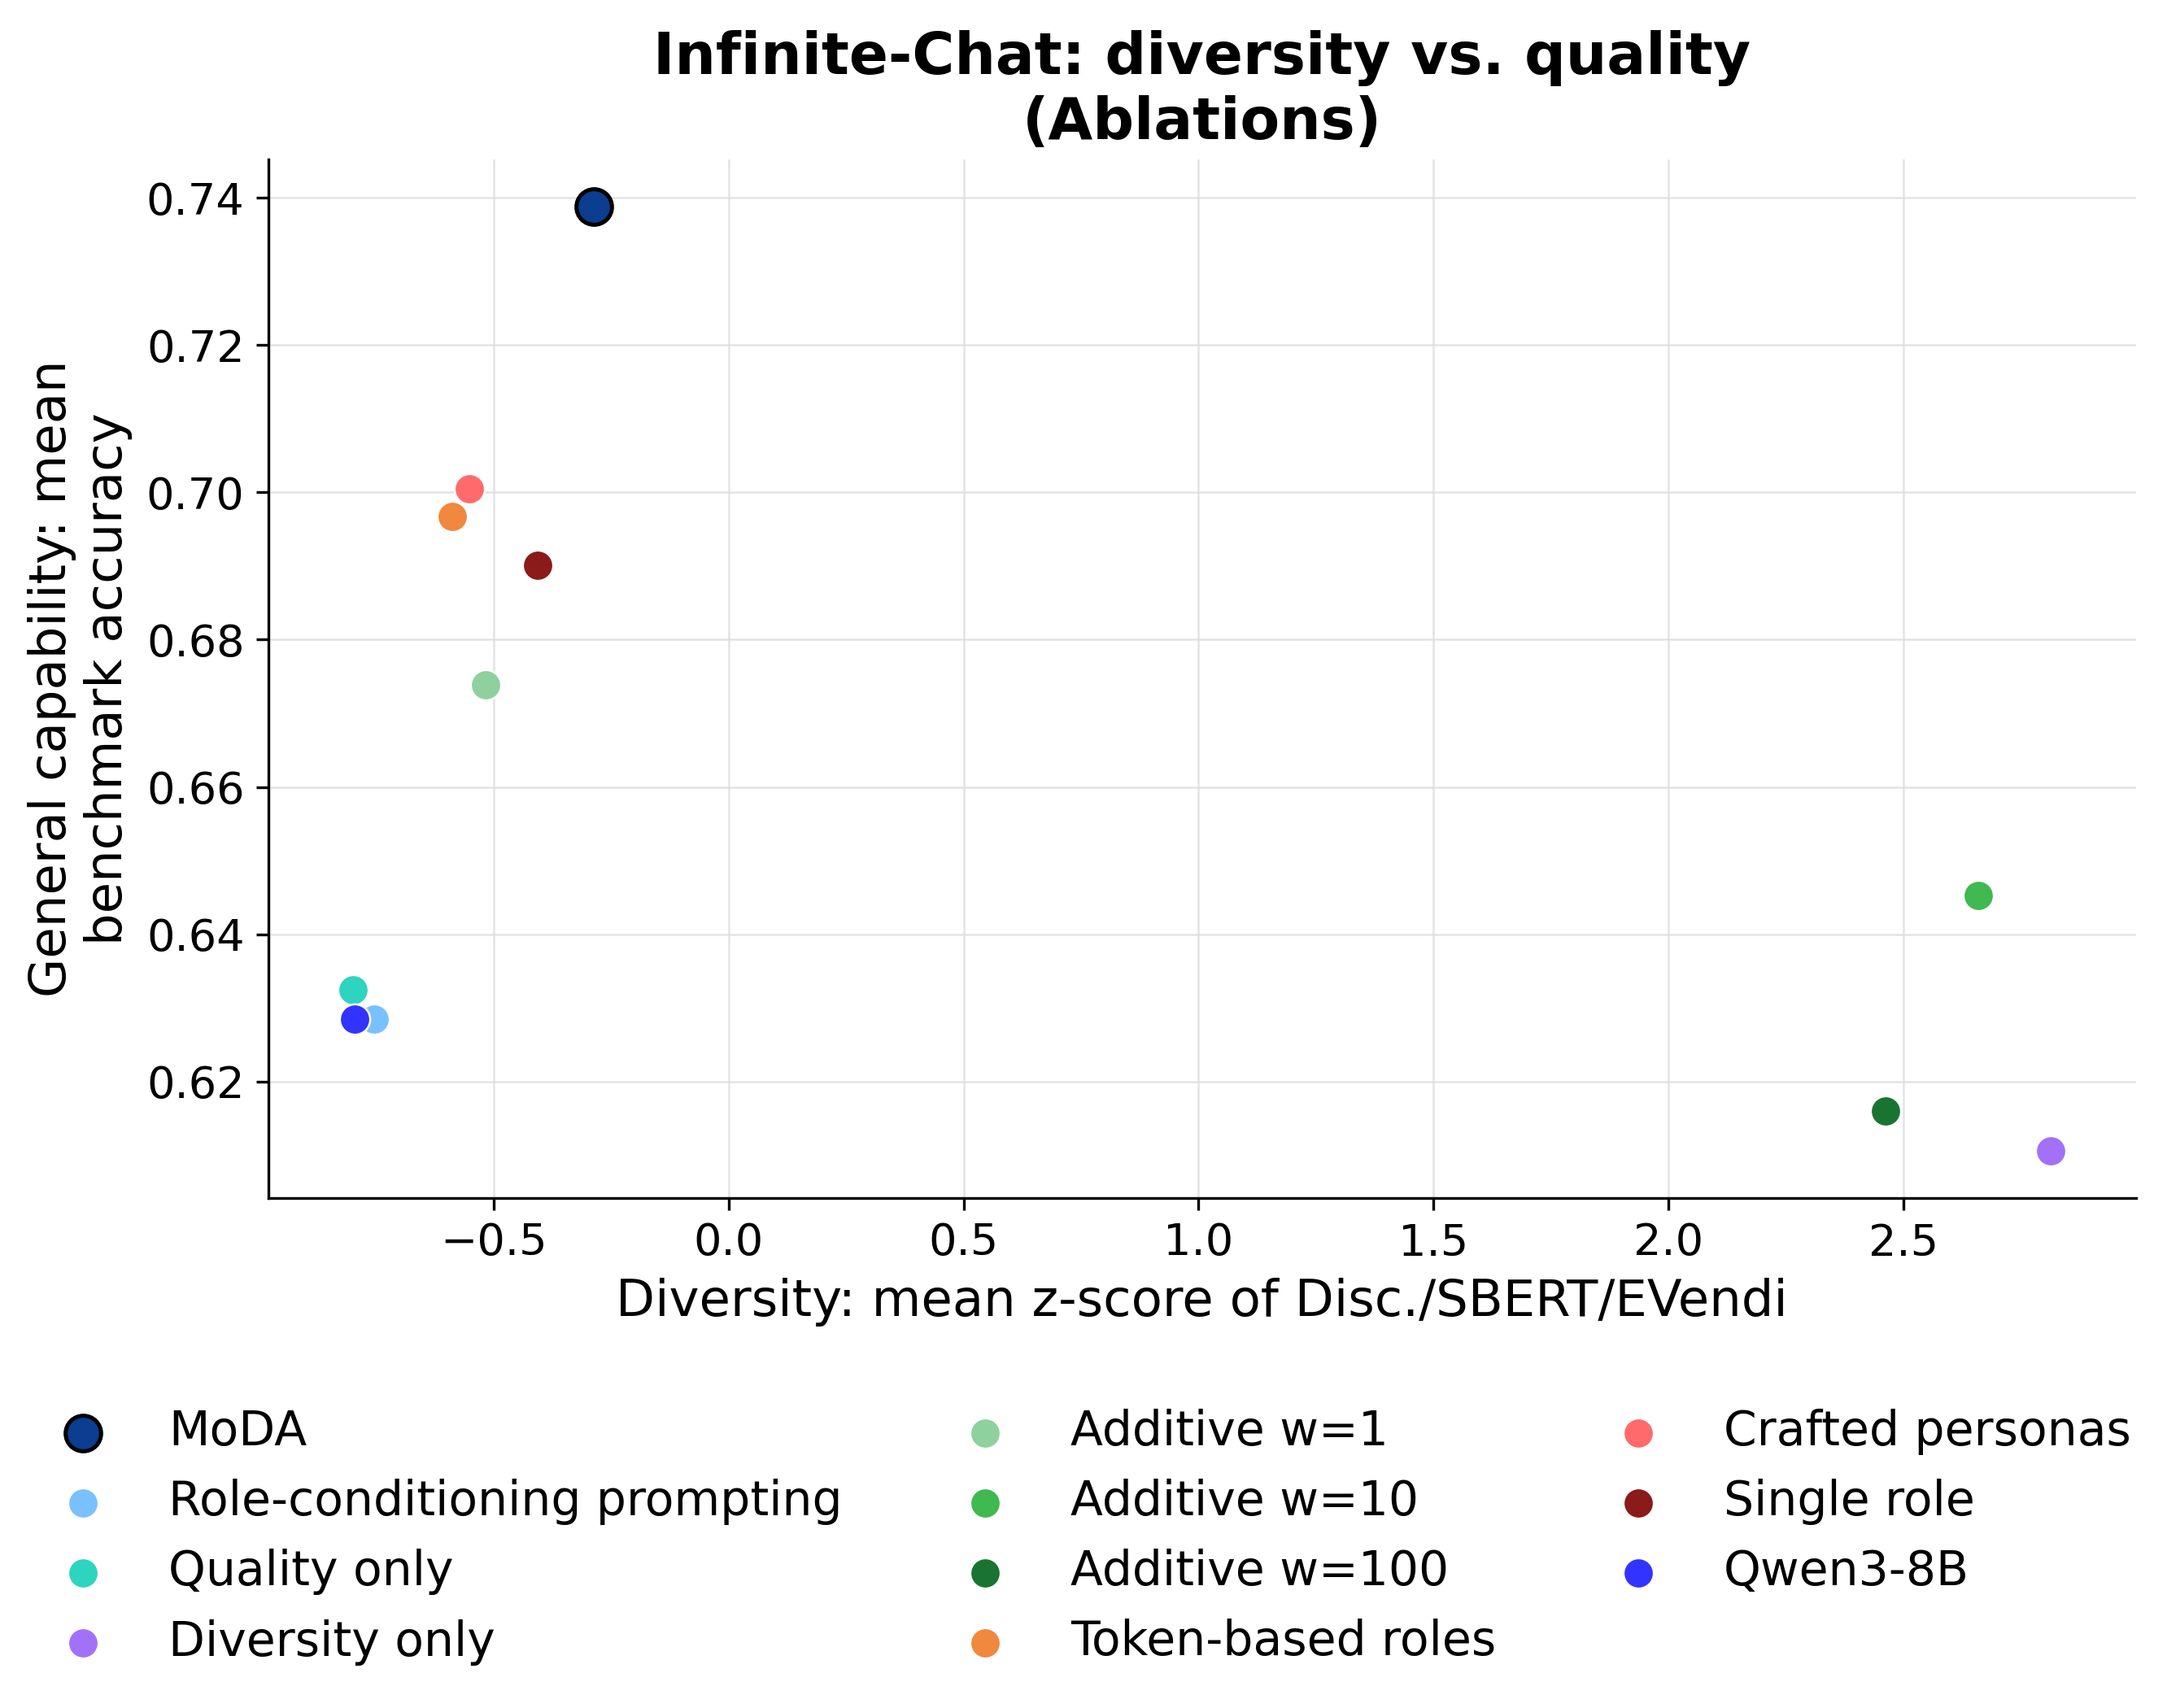
\includegraphics[width=\linewidth]{figures/pareto_infinite-chat_quality_ablations_composite.png}
  \small (b) Ablation variants
  \label{fig: domain application pareto ablations}
\end{minipage}
\caption{\textbf{Quality-diversity pareto front (Qwen3-8B, thinking disabled) baselines and ablated variants.} The x-axis is Infinite-Chat response diversity (mean z-score of Disc./SBERT/EmbVendi) and the y-axis is general capability (mean benchmark accuracy). \textbf{(a)} \method{} Pareto-dominates all the baselines, achieving better diversity and quality simultaneously. Results for Qwen3-8B (thinking enabled) and Llama-3.1-8B / GLM-4-9B (thinking disabled) are shown in Appendix~\ref{appx:generative diversity evaluation}. \textbf{(b)} The same comparison across \method{}'s ablated variants.}
\label{fig: domain application pareto}
\end{figure}

\begin{table*}[t]
\centering
\setlength{\tabcolsep}{3pt}
\resizebox{\textwidth}{!}{%
\begin{tabular}{lccccccccccccccccccc}
\toprule
Model & \multicolumn{4}{c}{\textit{Infinite-Chat}} & \multicolumn{4}{c}{\textit{NoveltyBench}} & \multicolumn{4}{c}{\textit{HypoBench}} & \multicolumn{4}{c}{\textit{PreScience}} & \multicolumn{3}{c}{Avg.} \\
\cmidrule(lr){2-5} \cmidrule(lr){6-9} \cmidrule(lr){10-13} \cmidrule(lr){14-17} \cmidrule(lr){18-20}
 & Disc. & SBERT & E-V & Qual.(\%) & Disc. & SBERT & E-V & Qual & Disc. & SBERT & E-V & Qual. & Disc. & SBERT & E-V & Qual. & Disc. & SBERT & E-V \\

\midrule
\multicolumn{9}{l}{\textsc{\underline{Qwen3-8B base, thinking disabled}}} \\
Qwen3-8B & 0.400 & 0.132 & 1.83 & 62.9  & 0.493 & 0.224 & 2.36 & 4.58 & 0.384 & 0.144 & 1.91 & \textbf{4.03} & 0.431 & 0.155 & 1.94 & \textbf{4.25} & 0.427 & 0.164 & 2.01 \\
DARLING (Mix) & \underline{0.430} & 0.203 & 2.33 & 57.9  & 0.513 & 0.281 & 2.96 & \underline{5.24} & 0.406 & \underline{0.222} & \underline{2.48} & 3.44 & \textbf{0.559} & \textbf{0.541} & \textbf{4.73} & 2.33 & \underline{0.477} & \underline{0.312} & \underline{3.12} \\
DARLING (WildChat) & 0.416 & 0.185 & 2.15 & 62.7  & 0.480 & 0.335 & 3.11 & 4.00 & 0.415 & 0.205 & 2.34 & 3.73 & 0.446 & 0.192 & 2.21 & \underline{4.03} & 0.439 & 0.229 & 2.45 \\
DivPO & 0.410 & \underline{0.274} & \underline{2.86} & \underline{66.2}  & \underline{0.519} & \underline{0.380} & \underline{3.58} & 4.87 & \underline{0.427} & 0.198 & 2.30 & \underline{3.89} & \underline{0.455} & \underline{0.233} & \underline{2.41} & 3.96 & 0.453 & 0.271 & 2.79 \\
\method & \textbf{0.472} & \textbf{0.482} & \textbf{4.40} & \textbf{73.2}  & \textbf{0.537} & \textbf{0.470} & \textbf{4.19} & \textbf{5.47} & \textbf{0.480} & \textbf{0.547} & \textbf{4.91} & 3.80 & 0.440 & 0.176 & 2.10 & 3.96 & \textbf{0.482} & \textbf{0.419} & \textbf{3.90} \\
\midrule
\multicolumn{9}{l}{\textsc{\underline{Qwen3-8B base, thinking enabled}}} \\
Qwen3-8B & 0.400 & 0.136 & 1.85 & 75.8  & 0.510 & 0.258 & 2.67 & \underline{4.90} & 0.399 & 0.164 & 2.05 & \textbf{3.93} & 0.441 & 0.136 & 1.83 & \underline{3.79} & 0.438 & 0.174 & 2.10 \\
SSoT & 0.397 & 0.178 & 2.09 & \underline{76.3}  & 0.438 & 0.239 & 2.57 & 0.46 & \underline{0.419} & \underline{0.220} & \underline{2.33} & 3.75 & \textbf{0.461} & \textbf{0.281} & \textbf{2.39} & 3.30 & 0.429 & \underline{0.230} & 2.34 \\
DivPO & \underline{0.414} & \underline{0.200} & \underline{2.20} & 71.7  & \underline{0.521} & \underline{0.327} & \underline{3.12} & \textbf{5.06} & 0.409 & 0.162 & 2.04 & \underline{3.89} & \underline{0.448} & 0.185 & 2.04 & \textbf{3.87} & \underline{0.448} & 0.218 & \underline{2.35} \\
\method & \textbf{0.600} & \textbf{0.909} & \textbf{9.04} & \textbf{76.8}  & \textbf{0.589} & \textbf{0.800} & \textbf{7.63} & 3.39 & \textbf{0.579} & \textbf{0.875} & \textbf{8.06} & 3.71 & 0.439 & \underline{0.194} & \underline{2.10} & 3.68 & \textbf{0.552} & \textbf{0.695} & \textbf{6.71} \\

\multicolumn{20}{l}{\textsc{\underline{{Llama-3.1-8B base, thinking disabled}}}} \\
Llama-3.1-8B & 0.414 & 0.217 & 2.40 & 46.7  & 0.512 & 0.312 & 3.04 & 4.80 & \textbf{0.469} & 0.207 & 2.38 & 3.60 & 0.461 & \textbf{0.514} & 3.67 & \textbf{2.62} & \textbf{0.464} & 0.312 & 2.87 \\
\method{} (Llama-3.1-8B) & \textbf{0.441} & \textbf{0.373} & \textbf{3.77} & \textbf{51.9}  & \textbf{0.532} & \textbf{0.392} & \textbf{3.75} & \textbf{6.17} & 0.410 & \textbf{0.324} & \textbf{3.27} & \textbf{3.65} & \textbf{0.472} & 0.470 & \textbf{3.89} & 2.54 & \textbf{0.464} & \textbf{0.390} & \textbf{3.67} \\
\midrule
\multicolumn{20}{l}{\textsc{\underline{GLM-4-9B base, thinking disabled}}} \\
GLM-4-9B & 0.421 & 0.234 & 2.60 & 44.9  & \textbf{0.544} & 0.408 & 4.08 & \textbf{4.14} & 0.402 & 0.225 & 2.52 & \textbf{3.75} & 0.461 & 0.438 & 4.15 & 2.57 & 0.457 & 0.326 & 3.34 \\
\method{}(GLM-4-9b) & \textbf{0.481} & \textbf{0.528} & \textbf{5.14} & \textbf{60.7}  & 0.502 & \textbf{0.521} & \textbf{5.01} & 2.70 & \textbf{0.452} & \textbf{0.485} & \textbf{4.64} & 3.68 & \textbf{0.464} & \textbf{0.448} & \textbf{4.28} & \textbf{2.58} & \textbf{0.475} & \textbf{0.495} & \textbf{4.77} \\
\bottomrule
\end{tabular}
}
\caption{Per-domain diversity (Disc. = discriminator diversity, SBERT = SBERT embedding pairwise distance, E-V = E-Vendi score) and quality (Qual.), averaged over $n{=}3$ random seeds. Infinite-Chat quality is general capability accuracy (\%); all other domains use the native quality score. Bold marks the best value within each model group. Table with error bar can be found in Appx \ref{appx:generative diversity evaluation}.}
\label{tab:domain-app-diversity-main}
\end{table*}




\textbf{General Capability Retention.} As shown in Figure \ref{fig:general capability retention}, our model achieves the best overall average pass@1, pass@5 and pass@10 score for general capability retention across thinking settings and base models among all baselines. With Qwen3-8B base and thinking disabled, it matches or exceeds the base model on 5 out of 7 benchmarks and achieves the best score among all baselines on 4 of them on pass@1 accuracy. Notably, with the GLM-4-9B base, \method improves average pass@1 by 15.8 percentage points, including a 3.89x relative improvement on GSM8K and a 2.37x relative improvement on MMLU. These results suggest that our method is an effective alignment approach that preserves, and in several cases significantly improves, the model's capabilities. We note that the language mixing penalty is important to maintain quality in some cases; without it, quality drops due to reward hacking from language mixing.


%We attribute this to the language-mixing penalty applied during training, which addresses the base model's native language-mixing issue. These results suggest that our method is an effective alignment approach that preserves, and in several cases significantly improves, the model's general capabilities.

\begin{figure}[ht]
\centering
\begin{minipage}[ht]{0.6\linewidth}
  \centering
  \resizebox{\linewidth}{!}{%
  \begin{table}[H]
\small
\setlength{\tabcolsep}{2.5pt}
\centering
\begin{tabular}{l*{7}{>{\centering\arraybackslash}p{0.95cm}}|>{\centering\arraybackslash}p{0.95cm}}
\toprule
Model & GSM8K & MMLU & GPQA & BoolQ & HS & TQA & IFEval & Avg. \\
\midrule
\multicolumn{9}{l}{\textsc{\underline{Qwen3-8B base, thinking disabled}}} \\
Qwen3-8B & \underline{84.5} & \textbf{82.0} & \underline{41.4} & 83.1 & 48.4 & 22.2 & \textbf{78.4} & 62.9 \\
DARLING (Mixture) & 63.5 & 63.0 & 34.3 & 76.7 & 62.2 & \underline{52.4} & 53.0 & 57.9 \\
DARLING (WildChat) & 77.9 & 55.0 & 34.3 & \textbf{86.4} & \underline{68.8} & 43.2 & 73.0 & 62.7 \\
DivPO & 80.5 & \underline{81.0} & 40.4 & 83.5 & 62.8 & 37.7 & \underline{77.3} & \underline{66.2} \\
\method & \textbf{86.7} & \underline{81.0} & \textbf{52.0} & \underline{84.8} & \textbf{73.4} & \textbf{57.9} & 76.9 & \textbf{73.2} \\
\midrule
\multicolumn{9}{l}{\textsc{\underline{Qwen3-8B base, thinking enabled}}} \\
Qwen3-8B & \textbf{90.3} & \textbf{94.0} & 43.4 & \textbf{87.2} & 70.9 & 64.9 & \textbf{79.7} & 75.8 \\
SSoT & 84.3 & \underline{93.0} & \textbf{55.1} & \textbf{87.2} & \textbf{80.1} & \textbf{72.8} & 61.9 & \underline{76.3} \\
DivPO & \underline{84.9} & 91.0 & 44.4 & \underline{83.2} & 65.0 & 55.3 & 77.6 & 71.7 \\
\method & 83.9 & \underline{93.0} & \underline{50.5} & \textbf{87.2} & \underline{76.2} & \underline{67.2} & \underline{79.5} & \textbf{76.8} \\
\midrule
\multicolumn{9}{l}{\textsc{\underline{Llama-3.1-8B base, thinking disabled}}} \\
Llama-3.1-8B & 71.3 & 16.0 & 6.1 & \textbf{81.6} & 30.2 & 53.4 & 68.8 & 46.7 \\
\method(Llama-3.1-8B) & \textbf{74.9} & \textbf{30.0} & \textbf{18.7} & 75.6 & \textbf{38.5} & \textbf{54.7} & \textbf{70.8} & \textbf{51.9}\\
\midrule
\multicolumn{9}{l}{\textsc{\underline{GLM-4-9B base, thinking disabled}}} \\
GLM-4-9B & 21.8 & 35.0 & 19.7 & 74.5 & \textbf{68.0} & \textbf{44.8} & 50.3 & 44.9  \\
\method(GLM-4-9B) & \textbf{84.9} & \textbf{83.0} & \textbf{33.3} & \textbf{81.2} & 52.3 & 34.5 & \textbf{55.5} & \textbf{60.7} \\
\bottomrule
\end{tabular}
\vspace{4pt}
\caption{General capability retention (Pass@1 accuracy \%), averaged over $n=3$ random seeds. Bold marks the best value within each model group; underline marks the second-best value within the Qwen3-8B groups. Table with error bar can be found in Appendix \ref{appx:general capability retention} Table \ref{tab:general-capability-pass1-error-bar}.}
\label{tab:general-capability-pass1}
\end{table}%
  }
\end{minipage}\hfill
\begin{minipage}[ht]{0.38\linewidth}
  \centering
  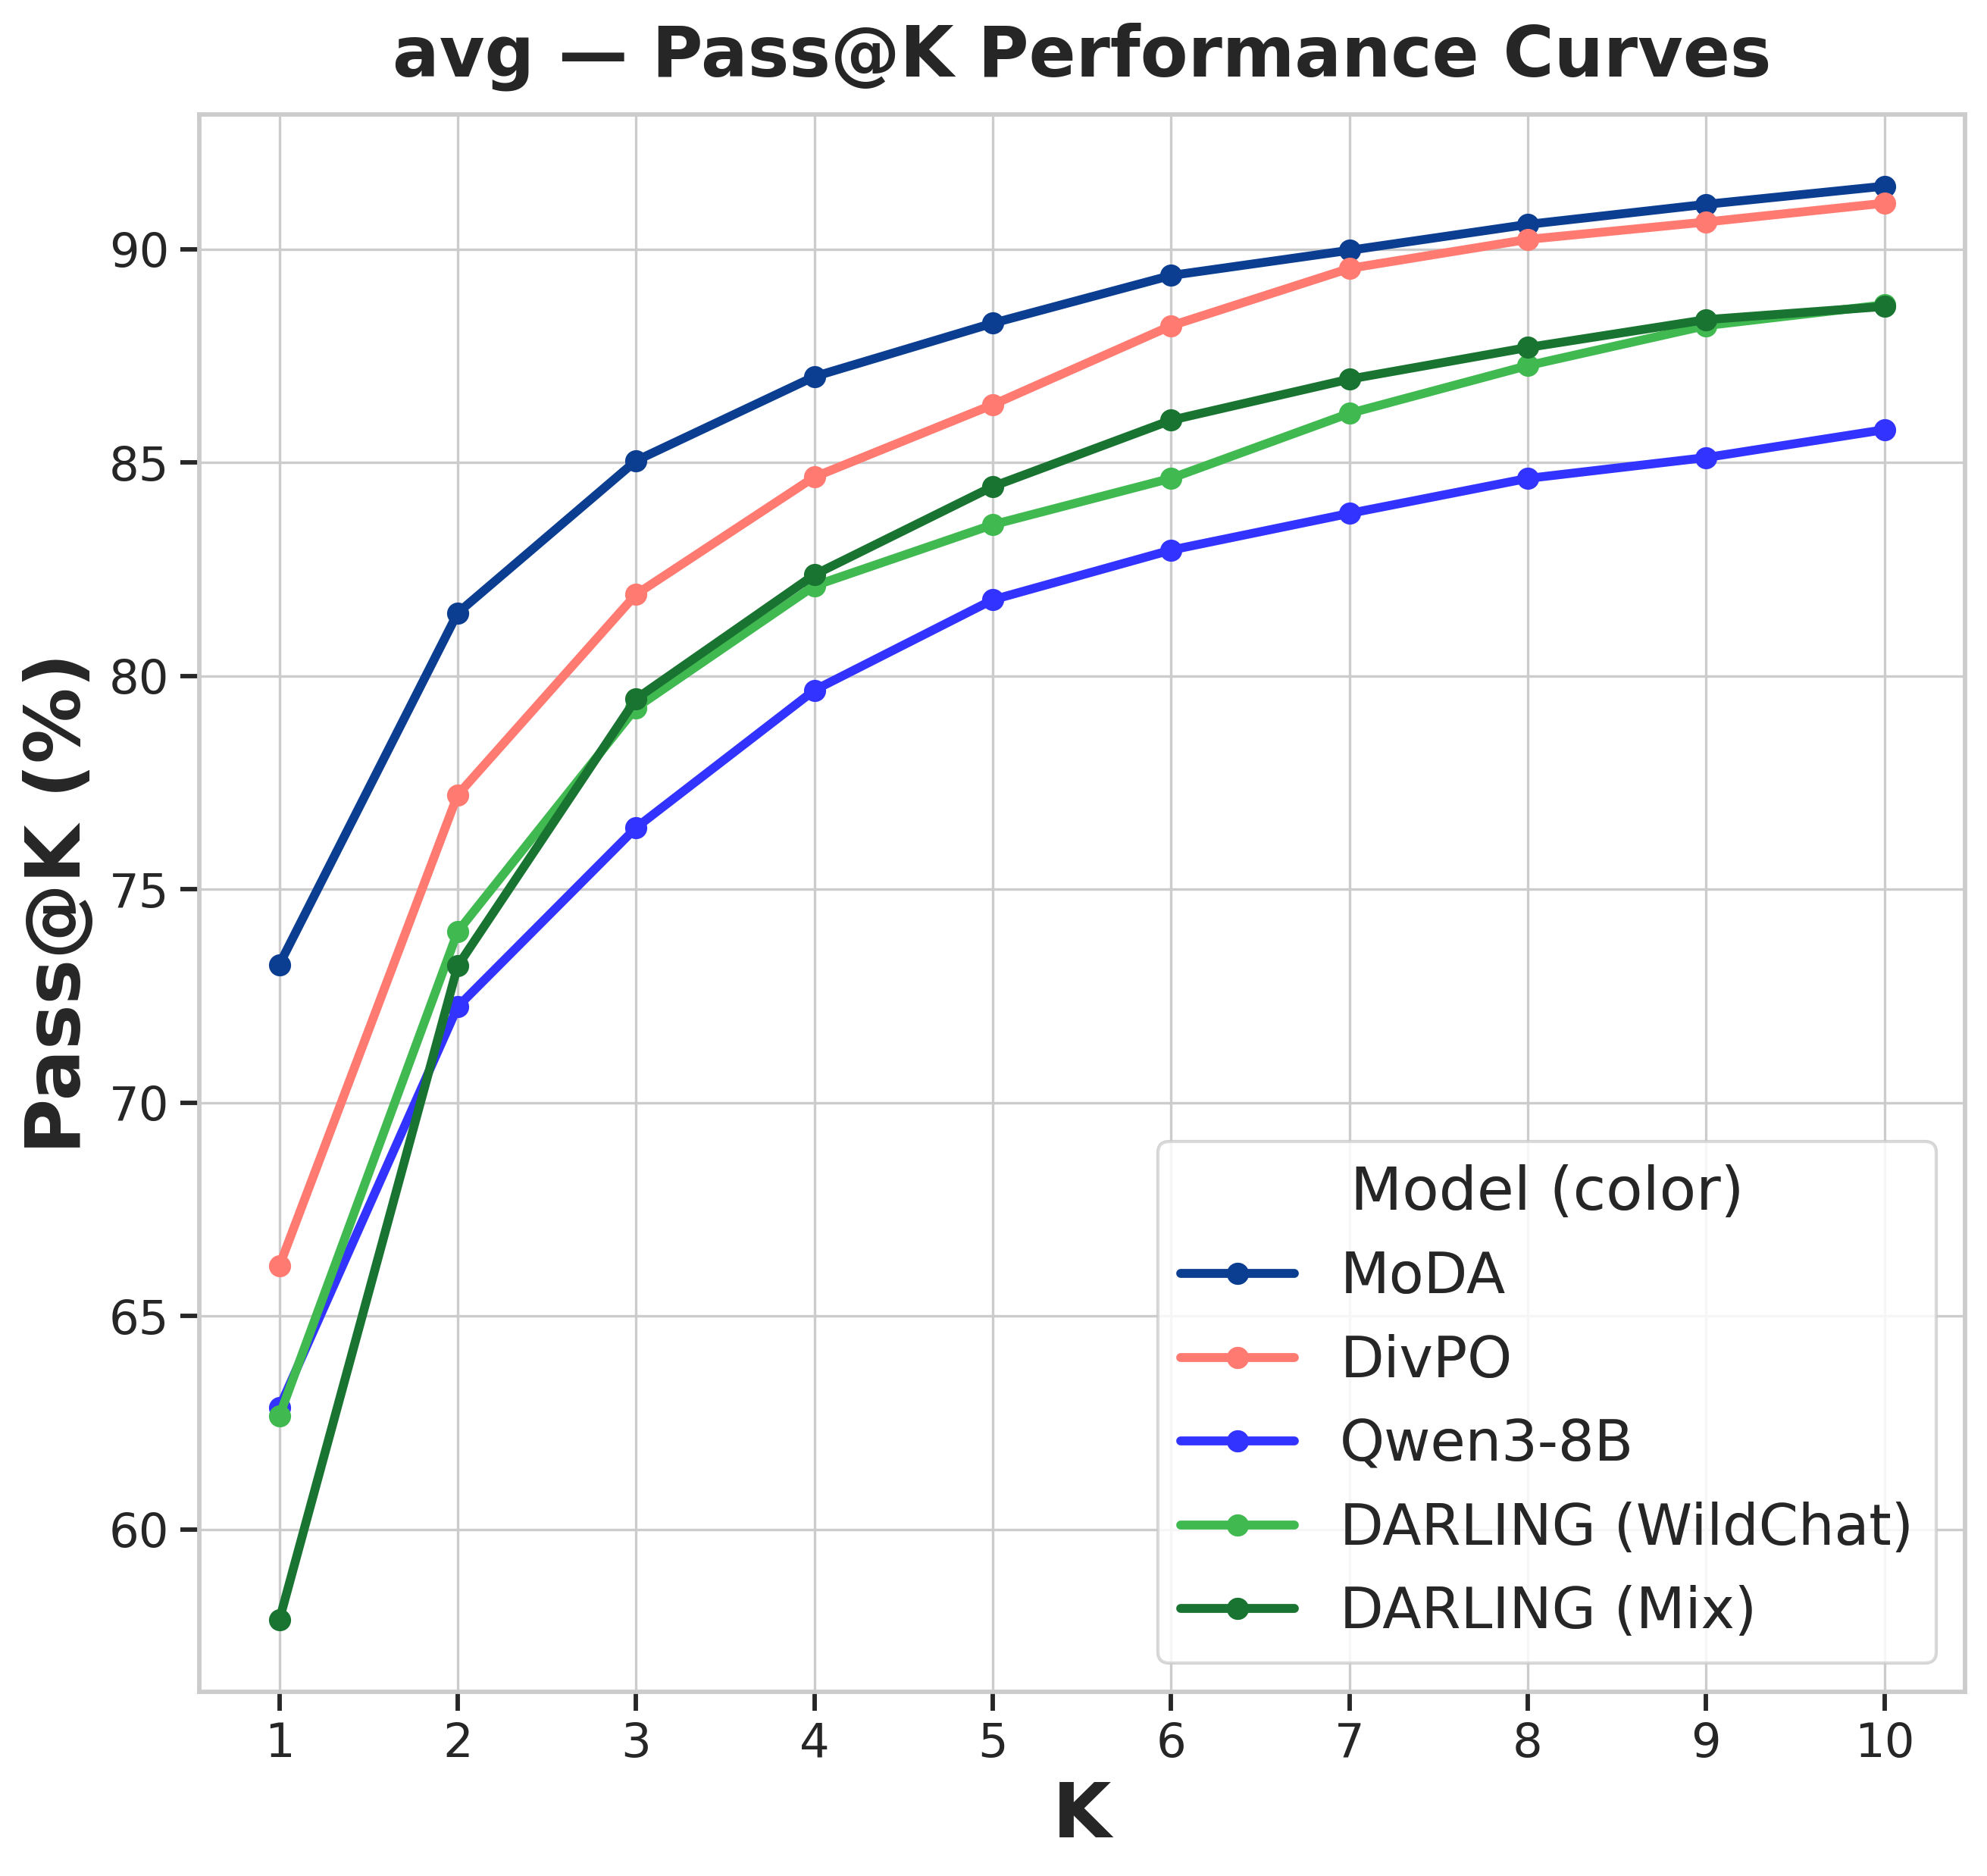
\includegraphics[width=\linewidth]{figures/main_pass_k/pass_at_k_figures/pass_at_k_avg_thinking_false_base_model_qwen3-8b.png}
\end{minipage}
\caption{\textbf{Left: General capability retention (Pass@1 accuracy \%)}, averaged over $n=3$ random seeds. Bold marks the best value within each model group; underline marks the second-best value within the Qwen3-8B groups. Table with error bar can be found in Appendix \ref{appx:general capability retention} Table \ref{tab:general-capability-pass1-error-bar}. \textbf{Right: General capability retention: pass@k accuracy.} Qwen3-8B base, thinking disabled models on the general capability suite average. Per-benchmark results are shown in Appendix \ref{appx:general capability retention} Figure \ref{fig:general capability pass@k thinking disabled}.}
\label{fig:general capability retention}
\end{figure}


% \begin{table}[H]
% \centering
% \small
% \setlength{\tabcolsep}{4pt}
% \begin{tabular}{lrrrr}
% \toprule
% Model Variant & HypoBench $\uparrow$ & PreScience $\uparrow$ & NoveltyBench $\uparrow$ & Infinite-Chat $\uparrow$ \\
% \midrule
% Base (No Thinking) & \textbf{4.025 $\pm$ 0.124} & \textbf{4.150 $\pm$ 0.191} & 4.403 & 0.514 $\pm$ 0.019 \\
% Ours (No Thinking) & 3.816 $\pm$ 0.075 & 3.602 $\pm$ 0.230 & \textbf{5.826} & \textbf{0.661 $\pm$ 0.018} \\
% \midrule
% Base (Thinking) & 3.920 $\pm$ 0.159 & 1.928 $\pm$ 0.206 & 3.147 & 0.497 $\pm$ 0.019 \\
% \ssot (Thinking) & 3.825 $\pm$ 0.113 & 1.494 $\pm$ 0.147 & 2.743 & 0.614 $\pm$ 0.018 \\
% Ours (Thinking) & 3.904 $\pm$ 0.114 & 3.581 $\pm$ 0.278 & 4.082 & 0.457 $\pm$ 0.019 \\

% \bottomrule
% \end{tabular}
% \caption{Aggregate domain-application quality across HypoBench, PreScience, NoveltyBench, and Infinite-Chat. Values are means with standard errors where available; NoveltyBench reports a single official aggregate in this run. Higher is better, and bold indicates the best model in each column.}
% \label{tab:domain-app-quality-error-bars}
% \end{table}

\subsection{Qualitative Results}
\label{sec:qualitative results}
We observe several interesting patterns in our experiments. Figure~\ref{fig:moda + 40blue} visualizes responses to the prompt \textbf{``Name a shade of blue''} from Qwen3-8B, Qwen3-8B with \ssot, and \method{} with thinking disabled. Consistent with the quantitative results, \method{} produces a larger set of valid and distinct responses. Interestingly, although \method{} uses only abstract numbered roles rather than hand-crafted personas, the model sometimes learns role-specific behavioral patterns, suggesting that abstract mode conditioning can induce differentiated characteristics, learned via competitive multi-agent training, without manually specifying each role. Figure~\ref{fig:qualitative-example-books-main} shows that, when asked to name a well-received book, the base model produces the same answer, ``To Kill a Mockingbird,'' in all six samples, whereas \method{} produces six distinct titles; additional qualitative examples are provided in Appendix~\ref{appx: generation examples}.
\liweiaddressed{can we pick example so that we can show across dirrent roles the generations are creative and different, while for other models, resampling doesn't give sufficiently creative candidates?}

\begin{figure}[ht]
\centering
\begin{promptbox}
\small\textit{Name one well received book that often appears in top book lists.}
\end{promptbox}
\begin{minipage}[t]{0.24\linewidth}
\begin{respbox}{Sample 1}
One well-received book that often appears in top book lists is \textbf{To Kill a Mockingbird} by Harper Lee. It is a classic of American literature and has consistently ranked high in various lists.
\end{respbox}
\end{minipage}\hfill%
\begin{minipage}[t]{0.24\linewidth}
\begin{respbox}{Sample 2}
One well-received book that often appears in top book lists is \textbf{To Kill a Mockingbird} by Harper Lee. It is widely celebrated for its powerful themes of racial injustice, morality, and empathy.
\end{respbox}
\end{minipage}\hfill%
\begin{minipage}[t]{0.24\linewidth}
\begin{modarespbox}{Role 1}
\textbf{``The Night Fire''} by Michael Connelly. \textbf{Award-winning author}: known for his intelligent, fast-paced crime fiction.
\end{modarespbox}
\end{minipage}\hfill%
\begin{minipage}[t]{0.24\linewidth}
\begin{modarespbox}{Role 2}
\textbf{``The Night Circus''} by Erin Morgenstern. Known for its richly imaginative world-building and lyrical prose.
\end{modarespbox}
\end{minipage}
\caption{\textbf{Qualitative example of diverse generation.} \textbf{Left two:} Qwen3-8B repeats the same title across samples. \textbf{Right two:} \method{} under distinct numbered roles produces conceptually distinct titles for the same prompt. More samples in Appendix~\ref{appx: generation examples} Figure~\ref{fig:qualitative-example-books}.}
\label{fig:qualitative-example-books-main}
\end{figure}


\subsection{Ablation Studies.}
% \begin{table}[H]
\centering
\setlength{\tabcolsep}{3pt}
\resizebox{\textwidth}{!}{%
\begin{tabular}{lccccc}
\toprule
& \multicolumn{2}{c}{General capability (Avg., \%)} & \multicolumn{3}{c}{Infinite-Chat Diversity} \\
\cmidrule(lr){2-3} \cmidrule(lr){4-6}
Ablation & Standard mode & Diverse mode & Disc. & SBERT & E-Vendi \\
\midrule
Role-conditioned prompting & 62.9  & 56.6  & 0.403  & 0.145  & 1.90  \\
Quality only & 63.2  & 61.8  & 0.401  & 0.131  & 1.82  \\
Diversity only & 61.1  & 10.7  & \textbf{0.656}  & \textbf{0.993}  & \textbf{9.77}  \\
Additive $w{=}1$ & 67.4  & 68.0  & 0.422  & 0.204  & 2.33  \\
Additive $w{=}10$ & 64.5  & 5.7  & 0.632  & 0.976  & 9.64  \\
Additive $w{=}100$ & 61.6  & 5.4  & 0.621  & 0.970  & 8.75  \\
Token-based roles & 69.7  & 67.9 & 0.419 & 0.197 & 2.04 \\
Crafted personas & 70.1  & 66.1  & 0.421  & 0.194  & 2.24  \\
Single role & 69.0  & 69.9  & 0.428  & 0.239  & 2.57  \\
\midrule
Qwen3-8B & 62.9 & - & 0.400 & 0.132 & 1.83 \\
\midrule
\textbf{\method{}} & \textbf{73.2}  & \textbf{71.6}  & 0.444  & 0.257  & 2.69  \\
\bottomrule
\end{tabular}
}
\vspace{4pt}
\caption{\textbf{Ablation results} for general capability (Pass@1) under standard and diverse decoding (accuracy \%) and Infinite-Chat diversity ($n{=}3$ random seeds). Bold marks the best value per column.}
\label{tab:ablation}
\vspace{-0.6cm}
\end{table}
% In this section, we perform ablation studies on the design choices of \method. 

\paragraph{Ablation Setups.}
First, to understand whether the diversity improvement comes from training or solely from role injection, we inject numbered roles to the base model (\textbf{Role-conditioned prompting}). Second, to examine whether the diversity gains are driven by the explicit diversity reward or arise naturally from repeated sampling and RL optimization, we trained \method{} with \textbf{Diversity only} reward and \textbf{Quality only} reward. Third, to understand the effect of quality-gated diversity reward, we trained \method{} with additive reward of weighted sum of quality and diversity metrics, with diversity weight = 1, 10 and 100 (\textbf{Additive w=1\textbackslash10\textbackslash 100}). Finally, to understand the effect of the naive numbered role injection, we trained several variants of \method: (1) \textbf{Crafted personas}, which conditions the roles with manually crafted persona descriptions (e.g. ``You are a creative problem solver.''; (2) \textbf{Single role}, conditions with only one role; (3) \textbf{Token-based roles}\liweiaddressed{again I think we should change this name to something a bit more serious.}, conditions the role with a dummy token (e.g. ``Start your response with APPLE.''). More implementation details are in Appendix \ref{appx: ablation model implementations}. We evaluate each ablated variants for general capability under standard and diverse decoding, and application domain suite under diverse decoding, with full results in Appendix \ref{appx: ablation results}.

\liweiaddressed{add a paragraph title to this, like the follwing two paragraphs.}
\textbf{Quality-Diversity Trade-off.} As shown in Figure~\ref{fig: domain application pareto}b, \method{} achieves the best accuracy on the general capability suite among all variants. \method{} also achieves 77\% higher SBERT diversity and 41.6\% higher E-Vendi diversity than role-conditioning prompting alone, indicating that role-conditioning prompting by itself is insufficient to induce diverse generation. The quality-only variant regresses in diversity relative to role-conditioning prompting, suggesting that an explicit diversity objective is necessary for diversity gains. The diversity-only variant achieves the best diversity metrics overall, but with the lowest accuracy under standard decoding, and its performance collapses entirely under diverse decoding, indicating that explicit quality gating is critical to preserving response quality.

\textbf{Additive Aggregation.}\label{ablation: additive aggregation} Many existing works on quality-diversity optimization aggregate quality and diversity objectives using a weighted sum~\citep{mouret2015illuminatingsearchspacesmapping, Chen2025PosttrainingLL}. We compare our method with variants trained using an additive reward objective. We find that additive aggregation is highly sensitive to the diversity weight $\lambda_d$. at $\lambda_d=1$, the additive variant shows modest diversity improvement over the baseline, but substantially less than \method{}; at $\lambda_d=10$ and $\lambda_d=100$, diversity improves significantly, but at the cost of general capability performance under diverse decoding. In contrast, \method{} separates quality control from diversity optimization through the quality gate, making the reward less sensitive to coefficient scaling and enables faster iteration.

\textbf{Role Injection.}
\label{ablation: role injection}
Prior work has shown that manually designed prompts can induce different model
behaviors \citep{park2024generative, argyle2023out}. We therefore craft six personas and inject them into the system prompt instead of the abstract numbered roles, testing whether hand-designed personas provide a stronger diversity prior than the abstract numbered role used in the main setting. To isolate the effect of role multiplicity from role content, we train a single-role variant in which every response is generated under the same \textit{``You are Role 1.''} system prompt. To study the effect of the identity-based role, we train a token-based conditioning variant in which the system prompt instructs a token-based distinguishing signal (e.g. \textit{``Start your response with APPLE/BANANA/ORANGE.''}).
As shown in Table~\ref{tab:ablation}, all variants exhibit a slight diversity improvement over the base model, but their gains are smaller than \method{}'s, indicating that multiple abstract numbered identity-based role provides a more effective exploration space than all the ablated variants, without sacrificing generalization.